\begin{frame}{Grade inflation in the UK at 2020}
\begin{figure}
    \centering
    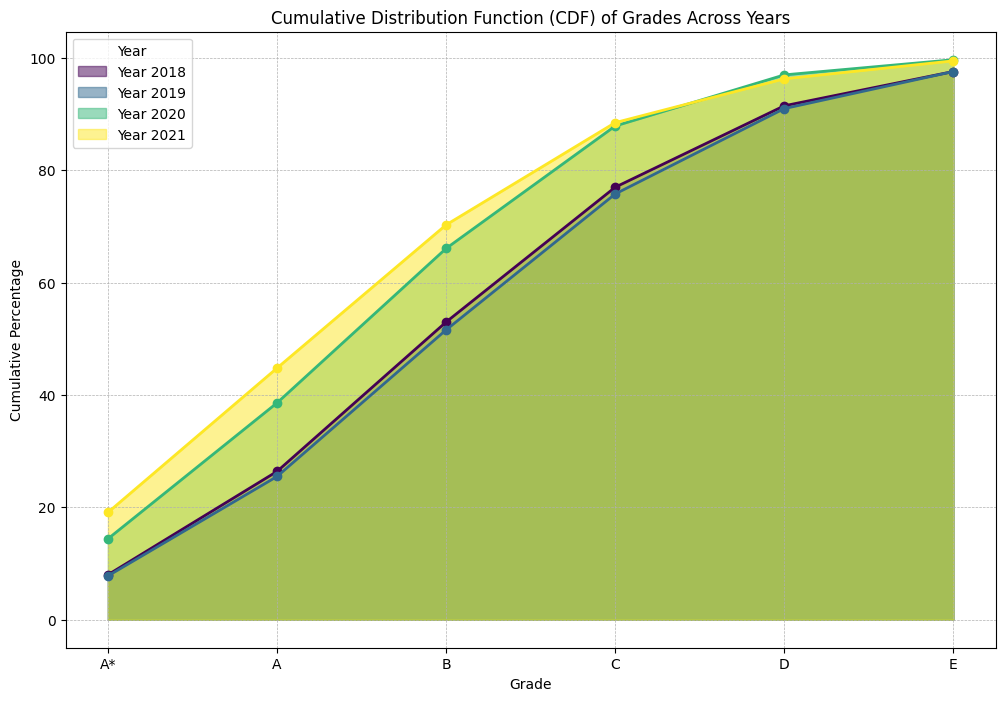
\includegraphics[width=\textwidth]{Figures/GradeDistribution.png}
    \label{fig:enter-label}
\end{figure}
\end{frame}

\begin{frame}{UK Higher Education Application System}
    \begin{itemize}
        \item Students take standardized in-person exams (A-Levels) to receive grades for university admission.

        \
        
        \item Students choose three subjects to take, each subject graded relative to other exam takers. 

        \

        \item Grades dictate students' final placement at universities.
        
        Universities send grade contingent offers to applicants before A-levels is finalized.

        Universities must abide by the offers they send.
        \end{itemize}
\end{frame}

\begin{frame}{Disruption in university admission system caused by COVID-19}
    \begin{itemize}
        \item On March 20, 2020\footnote{After application deadline (January 15th)}, the government canceled in-person exams due to COVID-19.

        \
        
        \item Instead, governments resorted to secondary schools to predict students A-levels score to use as the final grades.

        \

        \item Secondary schools assigned grades based on students' performance at school and past qualification exams.
    \end{itemize}
\end{frame}

\begin{frame}{Consequence of grade method change}
    \begin{itemize}
        \item Average final grades increase significantly after the grade method changed. Student placements improved for a majority of secondary schools.

        \

        \item Margin of grade improvement differed across subject groups.

    \end{itemize}
\end{frame}

\begin{frame}{Grade inflation in the UK at 2020}
\begin{figure}
    \centering
    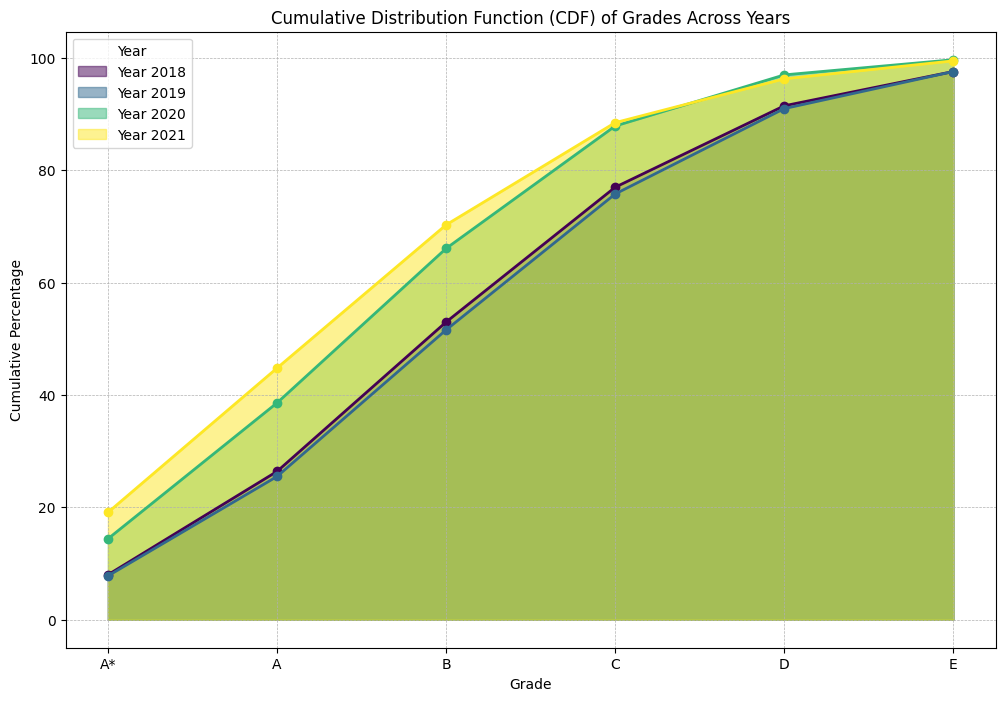
\includegraphics[width=\textwidth]{Figures/GradeDistribution.png}
    \label{fig:enter-label}
\end{figure}
\end{frame}

\begin{frame}{Consequence of grade method change}
    \begin{itemize}
        \item Competitive universities over-admitted students, changing demographics of the student body.

        \

        \item Example: Warwick Economics Department.
        
        \emph{Student Numbers (on Aug 11, 2022) · UG: 478 enrolled, 53 yet to enrol. The overshoot could be as high as 130. The target admission numbers were 400.  Final numbers will be known in a couple of weeks when enrolment is complete. The cumulative UG overshoot due to covid is now around 500. Admissions requirements have been tightened this year to address this. The offer will be raised to A* A* A.  Note that the previous year, roughly twice as many students showed up as were anticipated.}
    \end{itemize}
\end{frame}

\begin{frame}{Consequence of grade method change}
\begin{itemize}
    \item Students from elite-secondary schools occupied more spots at elite-universities in the subsequent years.
\end{itemize}
\end{frame}

\begin{frame}{Consequence of grade method change}
\begin{itemize}
    \item Rank Size Rule
    \begin{equation*}
        ln(Rank_j|TierX) = ln(GCSE_{j})\beta + \epsilon_{j}
    \end{equation*}
    $Rank_{j}$: Rank of school $j$ in sending students to Tier X universities.

    $GCSE_{j,t}$: Average performance of secondary-school at 2015.
\end{itemize}



\begin{figure}
    \centering
    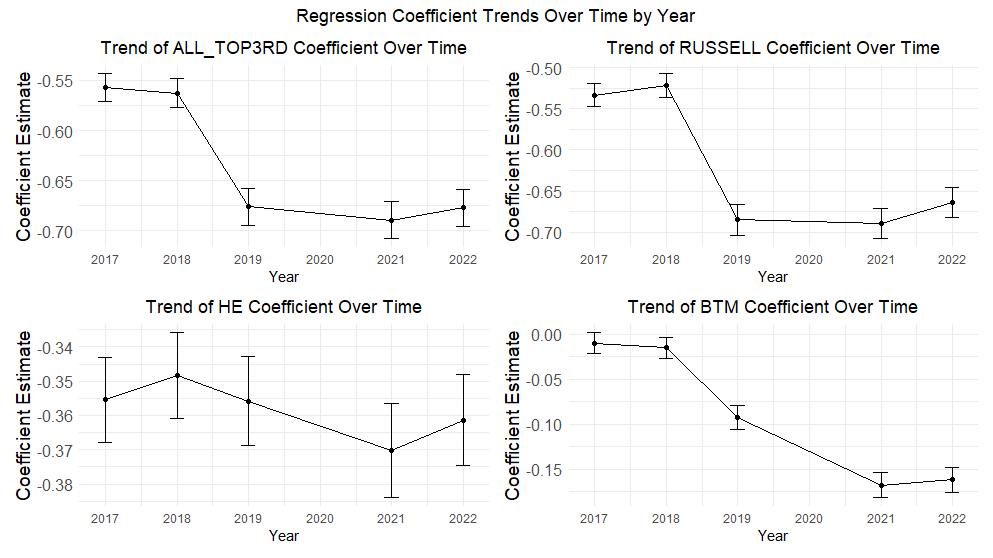
\includegraphics[width=0.8\textwidth]{Background/RankSizeRule.png}
    \label{fig:enter-label}
\end{figure}
* 2019 sample loses half of secondary school samples.
\end{frame}